%****************************************************
%	CHAPTER 6 - System Evaluation
%****************************************************

\chapter{Testing}
\label{ch:ch4}
A final version of the firmware is validated using the standards outlined in IEEE1012\footnote{IEEE Standard for System, Software, and Hardware Verification and Validation \cite{IEEE_STDVV}}. A series of unit tests were written to validate the subsystems and ensure that each module conforms to the outlined specification. Due to time constraints, rigorous data validation tests were not performed. In addition,IMU data and wave simulation testing will not be included.All subsystems are tested as a proof of concept using the unit tests outlined in the design methodology and the subsytem tests outlined in Appendix \ref{tab:UT001} to \ref{tab:UT008}. Finally, due to the 2020 COVID pandemic, final system evaluation could not be conducted in Antarctica. 

Once subsystem testing was completed, the following  full system tests were conducted

\begin{table}[H]
    \centering
    \caption{Description of accelerated system test protocol.}
    \begin{tabular}{|m{0.2\textwidth}|m{0.7\textwidth}|}
    \multicolumn{2}{l}{\textbf{SYS001} }\\
    \hline
    \textbf{Description} & Accelerated System Test\\
    \hline
    \textbf{Test Protocol:} &  The Buoy is fully assembled with all sensors connected and configured. The sample interval is set to 10 seconds with transmission occurring every 4 samples. Batteries are inserted and the device is placed inside the enclosure.The buoy is left outside in an area with an unobstructed view of the sky. The system is left to run for an hour and the incoming data is monitored through the Rock-block data portal.\\
    \hline
    \multicolumn{2}{l}{\textbf{SYS002} }\\
    \hline
    \textbf{Description} &  Power Test\\
    \hline
    \textbf{Test Protocol:} & The buoy was connected to an external power supply with all modules powered up and enabled. The INA219 power monitor was connected to an external data logger. The data logger measures the battery current, shunt voltage and load voltage of the system, The device was set with half an hour intervals and data was recorded for a single life cycle. The buoy was also set to output time-stamped state transitions to synchronise the current draw to each state of the system\\
    \hline
    \multicolumn{2}{l}{\textbf{SYS003} }\\
    \hline
    \textbf{Description} &  Freezer Test\\
    \hline
    \textbf{Test Protocol:} &  The Device was placed in a freezer for an hour to test the performance of the device in low temperatures. The device was modified to prevent transmissions from occurring. The freezer was set to $-20\degree C$  and the buoy status was visually monitored. After the test, the buoy was placed in a room-temperature environment where another accelerated test was performed.\\
    \hline
    \multicolumn{2}{l}{\textbf{SYS004} }\\
    \hline
    \textbf{Description} &  Full System Test\\
    \hline
    \textbf{Test Protocol:} &  All modules were assembled and the buoy placed in a power off state. The sample frequency was set to once every 30 minutes with IMU data logging every 2 hours. At the end of the sample period, the device transmitted two data packets: 4 x drift data packets and 1 x IMU data packet. The data was monitored through the rock-block message portal. \\
    \hline
    
    \end{tabular} 
    \label{tab:test_Systemtest_descrip}
\end{table}

\section{System Tests}
\label{sec:ch4_systests}
In this section, the results of the system tests outlined in Appendix \ref{tab:AT_SYS_EV} are discussed.

\subsection{Power Test}

A power test was conducted to monitor the current consumption of the buoy in various states. The INA219 sensor was disconnected from the system and connected to a data logger which sampled the Bus Voltage, Shunt Voltage, Current and Power at a sample rate of 1Hz. The buoy sample interval was set to half an hour. The device was connected to a bench-top power supply and the supply voltage was set to 7.2V input with positive and negative leads connected to where the battery was. The device was placed in a location with partially-obstructed line of site and set to run for a full cycle. The Results in Appendix \ref{fig:test_pwr_cycle} shows the current consumption of the device over a single buoy period.


The average current consumption is calculated as follows:

\begin{equation}
    I_{avg} = \frac{1}{T}\int_{0}^{T}i(t)dt = \frac{1}{T}\sum_{k=0}^{N}i(k)\Delta t
\end{equation}

where the time step $\Delta t$ is 1Hz and $T $ is the total time taken for the buoy to complete 1 cycle. Then, The average current consumption and cycle duration was calculated for each phase in the buoy cycle. The results are shown in the table below

\begin{table}[H]
    \centering
    \begin{tabular}{|l|c|c|}
    \hline
    \textbf{Cycle Phase: } & \textbf{Phase Duration (s):} & \textbf{Average current (mA):}\\
    \hline
     Initialization State & 20 & 494.37 \\
     \hline
     1st Sample State & 45 & 97.79 \\
     \hline 
     1st Sleep State & 1797 & 115.00 \\
     \hline
     2nd Sample State & 8 & 127.96\\
     \hline
     2nd Sleep State & 1797 & 114.41\\
     \hline
     3rd Sample Sate & 7 & 128.17\\
     \hline
     3rd Sleep State & 1797 & 112.87\\
     \hline
     4th Sample State (incl IMU) & 12  &129.71 \\
     \hline
     Transmit State & 135 & 157.01 \\
     \hline
     \hline
     Full Cycle:    & 10033 & 114.09 \\
     \hline
     \hline
    \end{tabular}
    \caption{Average current draw (mA) and cycle}
    \label{tab:test_powtest_data}
\end{table}



\section{Remote Deployment}
\label{sec:ch4_remotedeployment}
Remote testing of the system was conducted in the Southern Ocean during the SCALE\footnote{Southern Ocean Seasonal Experiment \url{http://scale.org.za/}} Antarctica Expedition. 6 prototype systems were brought on-board and carried to the Weddel Sea with the objective of testing the suitability, basic sensing capabilities, remote communication capability and GPS signal acquisition capabilities.However, during the expedition, the initial power system began to experience instabilities resulting in system failiures. Due to time and resource constraints, alternative power supplies were made for 3 systems. 2 systems were deployed in the 1st and 2nd Marginal Ice Zone (MIZ1 and MIZ2) respectively with One system being deployed on the Helideck of the Ship. These systems were tested in the electronics lab before deployment. The device was deployed with a DS18B20 temperature sensor and a UBlox Neo-7m 

\begin{table}[H]
    \centering
    \caption{Table showing the parameters the GPS was configured with before deployment }
    \begin{tabular}{|l|c|}
    \hline
    \textbf{Model:} & Ublox Neo-7M \\
    \hline
       \textbf{Baud Rate:}  & 115200 bit/s \\
       \hline
       \textbf{Data bits:} & 8 \\
       \hline
       \textbf{stop bits:} & 1 \\
       \hline
       \textbf{parity:} & None \\
       \hline
       \textbf{Active Networks:} & GPS, GLONASS \\
       \hline
       \textbf{Satelites:} & 3 - 6 \\
       \hline
       \textbf{NMEA Messages:} & GLL, GSA, ZDA \\
       \hline
    \end{tabular}

    \label{tab:test_remotetest_gpsconfig}
\end{table}

\subsubsection{Deployment procedure}

The  Buoy was switched on and sealed in the enclosure which was fastened to the tripod and placed on the deck of the ship. The buoy was placed in a basket along with three crew members who were fastened to the basket with personal harnesses. The Basked was attached to a crane, hoisted over the side of the ship and lowered towards the surface of the ocean. The crew members then identified a suitable Ice floe to place the buoy on. The floe had to have a diameter greater than 2m and visually capable of supporting the weight of the buoy. Once an ice floe was selected, the basked was maneuvered to hover 1m above the desired location.Figure \ref{fig:deployment}  shows the deployment of the buoys in the Marginal Ice Zone using this procedure. 

\begin{figure}[H]
    \centering
    \begin{subfigure}[h]{0.3\textwidth}
    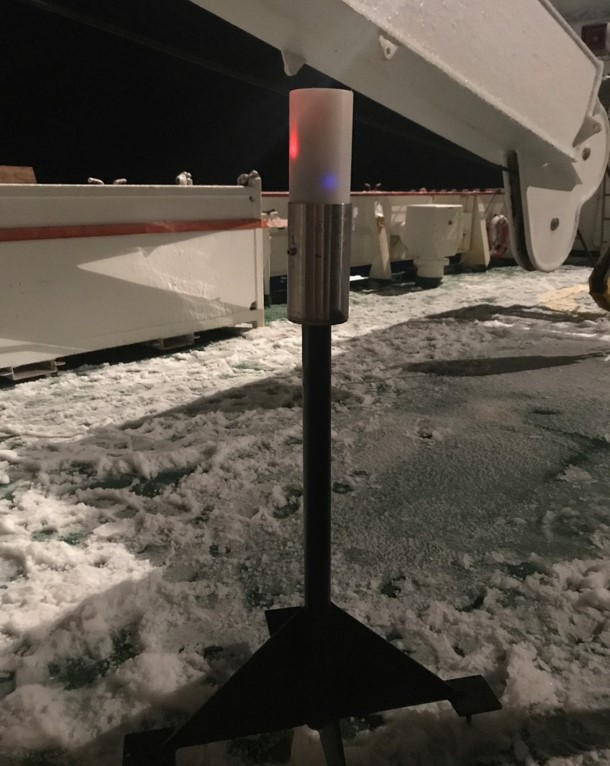
\includegraphics[width = 4cm,height = 6cm]{buoy.jpg}
    \caption{SHARC Buoy System}
    \end{subfigure}%
    \begin{subfigure}[h]{0.3\textwidth}
    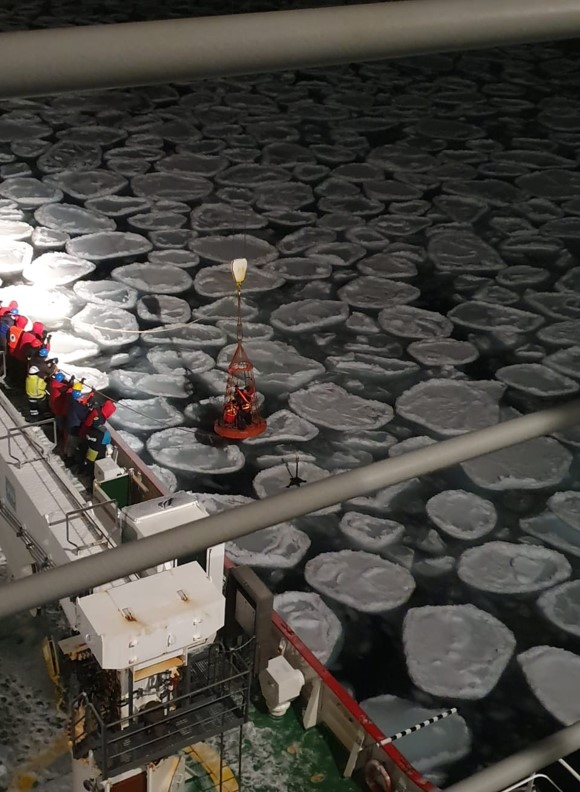
\includegraphics[width = 4cm,height=6cm]{basket.jpg}
    \caption{Deployment Proceedure}
    \end{subfigure}%
    \begin{subfigure}[h]{0.3\textwidth}
    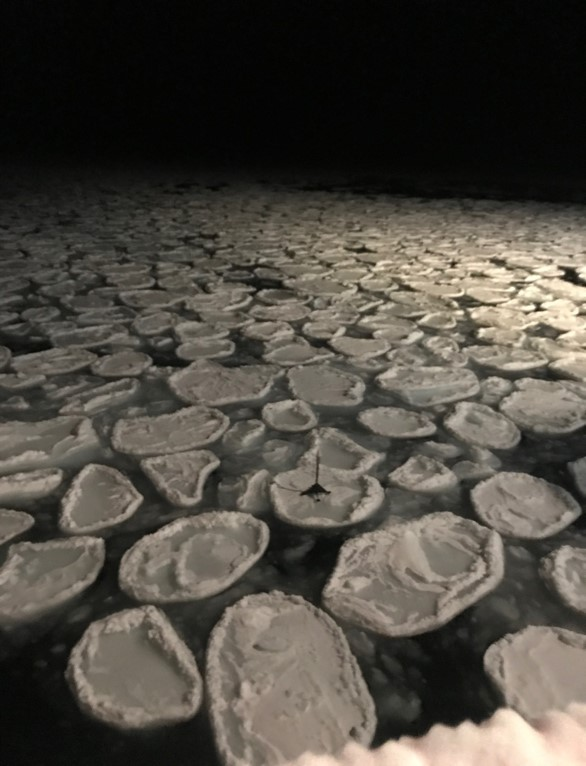
\includegraphics[width = 4cm,height=6cm]{deployment.jpg}
    \caption{Successful Deployment}
    \end{subfigure}%
    \caption{Figures Showing the  Fully Assembled SHARC Buoy device in a deployable state (a), The deployment procedure (b) and the results of a successful deployment showing a SHARC Buoy tethered to an Ice floe (c)}
    \label{fig:deployment}
\end{figure}
The buoy was then deployed from the basket with enough force for the spikes to penetrate into the sea ice thereby tethering the stand to the ice floe. Once complete, the buoy tracked GPS coordinates, signal diagnostic and ambient temperature. The conditions of the deployment are shown in the table below.
\begin{table}[H]
    \centering
    \caption{Deployment conditions for buoy 1 (2019-WC-SB01) and buoy 2 (2019-WC-SB02) including deployment coordinates, time and environmental conditions}
    \begin{tabular}{|l|l|l|}
    \hline
    Buoy Serial Number: & 2019-WC-SB01 & 2019-WC-SB02\\
    \hline
    Latitude: & $56\degree 59'59.70" S$ & $57\degree 17'11.28"$\\
    \hline
    Longitude: & $0\degree 0'36.96"E$ & $0\degree 1'18.30"E$\\
    \hline
    Date: & 26th July 2019 & 28th July 2019\\
    \hline
    Time: & 22h15 & 03h15\\
    \hline
    Air Temperature: & $-10.7 \degree C$ & $-17.5 \degree C$\\
    \hline
    \end{tabular}

    \label{tab:test_remotetest_Deployemt }
\end{table}

\subsubsection{Results}
\label{sec:ch4_results}

The First Buoy transmitted one message after deployment before losing contact. The second buoy failed to transmit any messages. The 3rd buoy survived on the helideck for 1 week. The batteries were then changed and the buoy continued to transmit data continuously. GPS data collected from the transmission packets was compared to the GPS data recorded from the ship and the results are shown in the figure Figure \ref{fig:test_deploymenttest_GPS}.


Figure \ref{fig:test_deploymenttest_temp}  shows the ambient temperature sampled by the buoy during its journey from Antarctica to East London. The data collected was compared to the data from the ship's on-board weather station.

\section{Final Evaluation}
\label{sec:ch4_final_eval}
The platform was evaluated both on a subsystem and full system level. Validation of the system occurred using the Acceptance tests AT001 to AT005 outlined in Chapter 3. Table \ref{tab:AT_SSYS_EV} shows the results of the acceptance tests and the traceability of the subsystems.\par

The full system was evaluated using Acceptance Tests AT007 to AT009. Due to project timeline constraints, rigorous calibration tests (AT006) could not be performed on all the required subsystems. The results of the Acceptance tests are shown in the table below.
\begin{table}[H]
    \centering
    \caption{Results of the full system acceptance tests indicated by a \checkmark in the appropriate column}
    \begin{tabular}{|c|c|c|c|}
    \cline{2-4}
    \multicolumn{1}{c|}{}&  \multicolumn{3}{|c|}{Full System Acceptance:} \\
    \hline
    \textbf{Unit Test:} & \textbf{Fully Satisfied:} & \textbf{Partially Satisfied:} & \textbf{Not satisfied:} \\
   \hline
    AT006 & & \checkmark & \\
    \hline
    AT007 & \checkmark & & \\
    \hline
    AT008 & &  \checkmark& \\
    \hline
    AT009 & & & \checkmark \\
    \hline
    \end{tabular}

    \label{tab:AT_SYS_EV}
\end{table}

Full system calibration was partially satisfied. The power monitor circuit was calibrated successfully for the power supply and the IMU successfully passed the self-test however, additional IMU calibrations could not be performed. The extent of IMU functionality demonstrated by this platform is to prove functionality by initializing and sampling at a fixed known rate. Long-term data logging and wave measurements fall outside the scope of this project.It is recommended for future research to create an acceptance test for extensive IMU calibrations. Finally pressure measurements are difficult to verify without a calibrated barometer. In future work, verification of the environmental sensor should be conducted at a location with a calibrated weather station.

The system successfully completed low temperature tests in a $-20\degree C$ freezer and could function normally afterwards. However, visual means (LED's, active visual monitoring) were used to monitor the performance in the freezer. In the future, more extensive low temperature tests should be conducted. An additional improvement is to link the device to a data-logger and conducted low-temperature data validation tests to ensure proper operation of the buoy in low temperatures.

\subsection{System Validation}
Once the testing was completed, the final system was evaluated against the system requirements. This ultimately proves if the steps undertaken in chapter 3 had successfully fulfilled the requirements outlined by the stakeholders and evaluate the achievements of the device. These results are shown in table \ref{tab:final_eval_funcreq} below.

\begin{table}[H]
    \centering
    \caption{Results of the platform evaluation and how each functional requirement was addressed.}
    \begin{tabular}{|m{0.15\textwidth}|c| m{0.7\textwidth}|}
    \hline
     Functional Requirement   &  Validation & Discussion\\
     \hline
     FR001 & Fully Met & \textit{The System shall have a protective enclosure against precipitation and frost}\\
          \hline
     FR002 & Fully Met &\textit{Enclosure shall be from strong, corrosion resistant materials with strong thermal Characteristics}\\
          \hline
     FR003 & Partially Met& \textit{The Device will protect electronics from internal humidity} - This requirement was partially met. When the device transitioned from sub zero temperatures to room temperature, condensation formed both inside and outside the device. While the electronics continued to work, this could result in unexpected failures and needs to be addressed in the next iteration.\\
          \hline
     FR004 & Fully Met & \textit{The Electronics will be elevated above the ground by 1 m to protect against freezing over}\\
          \hline
     FR005 &Fully Met & textit{System will transmit data via iridium modem}\\
          \hline
     FR006 &  Fully Met &\textit{System shall contain a global positioning (GNSS) device}\\
          \hline
     FR007 & Fully Met &\textit{device shall be battery powered} \\
          \hline
     FR008 & Fully Met &\textit{All Subsystems shall be rated for extreme temperatures}\\
          \hline
     FR009 & Fully Met& \textit{Device shall measure Ambient Temperature}\\
          \hline
     FR010 & Fully Met & \textit{Device shall measure Atmospheric Pressure}\\
          \hline
     FR011 & Partially Met &\textit{Device shall contain an Inertial Measurement Unit (IMU) to record acceleration (3-axes) and rotation (3-axes) of the ice floe.} - A proof of concept was implemented with the IMU capable of sampling all 6 axes for a total of 336 bytes of data. This is insufficient to calculate significant wave height.\\
          \hline
     FR012 & Fully Met & \textit{Device to contain sufficient memory for data storage}\\
          \hline
     FR013 & Fully Met &\textit{ Device to contain a processing unit to control sensors and process data}\\     
     \hline
     FR014 & Fully Met & \textit{ Device to be optimised for low-power consumption and power event handling}\\
          \hline
     FR015 & Unsatisfied & \textit{Device shall be factory calibrated prior to shipping and delivered in a state where it can be deployed at a moment's notice} - the sensors were insufficiently calibrated to fully meet this requirement.\\
          \hline
    FR016 & Fully Met & \textit{The Device will cost less than currently available systems.} - The overall cost for a single system is: R8,421.13 \\
    \hline
    \end{tabular}

    \label{tab:final_eval_funcreq}
\end{table}

\section{Discussion}
\label{sec:ch4_disc}

\subsection{Power Requirements}
\label{subsection:PWR}
The Initialization State is the most power intensive state drawing 494.37mA. This can be attributed to the Rockblock 9603 modem which draws 450mA to charge the on-board super capacitors. The effects of placing the modem to sleep can be seen throughout the data in Figure \ref{fig:test_pwr_cycle} and Table \ref{tab:test_powtest_data} where the average current barely increases above 130mA. The effects of putting the buoy to sleep mode when the device is inactive results in a significant drop in current consumption as Te average current consumed during sample mode is roughly 10-15mA larger than the current consumption during sleep mode. However, this is not true for the first sample state which results in the lowest current consumption at any point in the operational cycle of the buoy.\par The 4th sample state has the largest average current draw and the longest phase duration of all the sample states. This is to be expected as the inclusion of IMU sampling results in a longer data acquisition time as well as a higher current consumption. Finally, The Transmit state was expected to have the second highest current consumption since the Iridium modem was turned back on. At this point, the current draw increased to 250mA as shown in figure \ref{fig:test_pwr_cycle}. This occurred twice during the transmission phase. Despite this spike in consumption, the average current over the phase was 157.01mA despite multiple transmission attempts.A visual representation of the data in Table \ref{tab:test_powtest_data} is given in Appendix \ref{fig:test_powtest_avgcurr}

The duration of each state has a significant impact on the average current consumption of the buoy. While the initialization state current and the Transmission state had significantly higher current consumption, the phase duration of these states were significantly smaller than the sleep states. The long periods of inactivity dominated the power cycle resulting in an average current of 114.09mA. The duration of the sample states were small as a result of fast data acquisition and sampling speeds. However, the 1st sample state had the longest duration. This was due to a failure to acquire a GPS signal with 30 seconds which resulted in a timeout. The 4th Sample state also had a relatively long phase duration due to the inclusion of the IMU in the sample routine. Finally, the longest, active state was the Transmit State. During this state, multiple attempts were made to successfully transmit a packet of data and failed resulting in the relatively long phase duration. Overall, it took 10033 seconds or (2 hrs 47.217 min) whereas each sleep-state was found to be extremely consistent. This shows that the sample and transmit states have a non-negligible duration which can affect the accuracy of the sampling resulting in time delays and desynchronisations. This needs to be accounted for in the future.

\subsection{System Performance}

Figure \ref{fig:test_deploymenttest_GPS} shows that data collected from the Buoy's GPS correlated well with the data from the ship. However, large gaps appear in the Buoy's data-set. This can be attributed to signal loss or failure to acquire GPS position. In addition. the positional error appears larger for coordinates greater than $50\degree S$ and smaller as the trajectory approaches East London, This could suggest that the GPS satellite signal is much weaker closer to the Antarctic continent and may be attributed to either the strength of the antenna or the spread of GNSS satellites in the region.

Figure \ref{fig:test_deploymenttest_temp} shows that the temperature measured by the sensor was wildly inaccurate. This may be due to poor calibration of the sensor or external influences from the ship. Additionally, Missing packets resulted in large "spikes" in the data. The data, however does show a trend towards warmer temperatures which is also reflected by the ship data. Therefore, the sensor was able to characterise the change to warmer temperatures however, the data is too inaccurate to be valid. This data from version 1 of the buoy was captured with the DS18B20 thereby showing it was not practical for this application. The new sensor (BMP280) could not be verified by remote testing due to cancellations of the 2020 Antarctic expedition.

\subsection{Mechanical Features}

The mechanical features of the system successfully met the functional requirements FR001, FR002, FR004. FR003 was partially met as preliminary freezer tests resulted in condensation both inside and outside the system. In spite of this, the electronics continued to work however, a revision of the design should be made to reduce the internal humidity of the system when it transitions from a sub-zero environment to room temperature. \par 

The mechanical features of the system, while robust, were quite bulky and heavy. The stacked PCB design allowed for robust, modular development of the system and resulted in increased mechanical strength. However, the result was increased physical size of the device and increased cost. For future iterations, a single PCB with all the components should be created. By reducing reliance on off-the-shelf development boards, the performance, size and power consumption of the system can be more carefully controlled. More over, a single PCB design requires less physical hardware to secure the system to the enclosure such as Hex spacers, screws and washers. This can significantly reduce the price of fabrication. This design was also found to create points of failures within the device. By having separate PCBs, additional wires were required to connect the boards. If a wire loses contact or breaks, the device stops working. Finally, by reducing the electronics size, more batteries could be included which can provide more power for the system.

\subsection{Power System}

The power system was the largest constraint to the device. The physical size of the enclosure limited the number of batteries included in the system and therefore lifespan of the buoy. The initial decision was to use $LiSoCl_2$ D cell batteries.These were chosen for their high specific energy and low temperature resistance. 2 3.6V batteries were connected 2 in series and 2 in parallel resulting in 7.2V into the LDO. However, in low temperature environments, the internal resistance of the batteries dropped significantly resulting in system brownouts and unexpected resets. These were exchanged for AA $LiFeS_2$. These batteries had higher stability at lower temperatures at a cost of significantly reduced specific energy. In addition, 4 cells were required in parallel to produce the required voltage thereby increasing the battery requirement.\par 

The result was a maximum survivable period of 8 days in low temperatures $< 0 \degree C$ and 10 days in Standard temperature. The seasonal requirement for operation is at-least a month. In order to meet this requirement, the power system requires significant revision. The Average load current was estimated to be 114.09mA over a 2 hour cycle. for a period of 30 days, the total energy consumed is $114.09 \times (30 days) \times (24 hours)$ or $82,114.8mA$ Future improvements to meet this requirement would be to use batteries with higher specific energy, couple the power system with an energy harvester or use a rechargeable power source. Additionally, the load current can be reduced significantly by implementing more power saving features such as MOSFET switches to turn off unneeded sensors or configuring devices such as the GPS for power saving mode.

\subsection{Future work on wave measurements}

The IMU was successfully integrated into the project however, the sampling requirements resulted in extremely large data sets requiring complex data management algorithms. Morever, the constraints of the Iridium data buffer significantly impacted the type of data that could be transmitted. The recorded time series requires compression algorithms/software processing algorithms which fall outside the scope of this course. Therefore, in terms of the project goals, the IMU only partially satisfies the requirements and more firmware development is required for wave data measurements to become fully realisable.

The MPU6050 is a low cost, 6 axis inertial measurement. This more than satisfies the requirements for analysing waves in terms of spectra, co spectra and significant wave height. The majority of devices in the field use high precision, expensive IMUs with low cost devices similar to the MPU6050 to verify the measurements. This shows that there is still room for investigation into the accuracy and performance of low cost IMUs for complex functions. 

\subsection{Short-burst Data Modems vs Telephone modems}

The current version of the SHARC buoy uses a short-burst data modem with a maximum transmission buffer size of 340 bytes. This resulted in extreme data constraints which reduced the functionality of the system. Despite this complexity, the device was well integrated into the system and was able to reliably transmit data even through the enclosure. Short Burst Data is a very data limiting protocol and is not a feasible solution for real-time, raw IMU data. In future version, the Iridium 9522A would be a more feasible solution as the data buffer is much larger (1960 bytes). Alternatively, an iridium device with a sim card or continuous real time data transmission protocol.\par

The modem required the most design consideration. The device dominated the current sample and had the highest current consumption of all components. Therefore, the majority of software optimization was focused on optimizing the power cycle of the device. Despite having an extremely large current cycle, the average current consumption over a 2 hour cycle was reduced significantly therefore successfully meeting the functional requirements.

\subsection{Evaluation against the State of the Art}

The final evaluation for the system was against other devices in the field. Most of these devices have been field tested to a larger extent than this device and have a higher technological readiness level. Significantly more testing is required to verify the field performance against the operation of the system.\par

However, SHARC buoy consumes significantly less power than the majority of devices in the field. The mode supply voltage is 12V with some devices drawing up to 18V compared to the buoy's 7.2V operating voltage.\par 

Finally, while the SHARC buoy has more primitive modules on board, the device can, more evenly, measure a wider range of variables. Most devices generate complex measurements from single modules such as a high-powered IMU or AHRS measurement system. Devices such as WIIOS and WII buoy only contain low powered modules to compliment the measurements of the higher-powered components. This provides a unique opportunity for SHARC buoy to provide a deeper insight into performance optimization in this region.\par 

Overall, the system shows that it is unique and fits a niche as a low powered, modular sensing device however, more rigorous tests and calibrations are required to bring the device to an overall state of technological readiness.
